% Receiving antenna -> Thevenin equivalent (effective-area derivation, L2).
% Build: run scripts/circuits/build.sh  ->  book/extras/viz/img/recv-circuit.svg
\documentclass[border=6pt]{standalone}
\usepackage{circuitikz}
\usetikzlibrary{arrows.meta}
\definecolor{navy}{HTML}{004A85}
\definecolor{cblue}{HTML}{0067B9}
\definecolor{cred}{HTML}{B3213A}
\definecolor{camber}{HTML}{8A5A00}
\definecolor{cink3}{HTML}{5B6573}
\ctikzset{bipoles/thickness=1.1}
\begin{document}
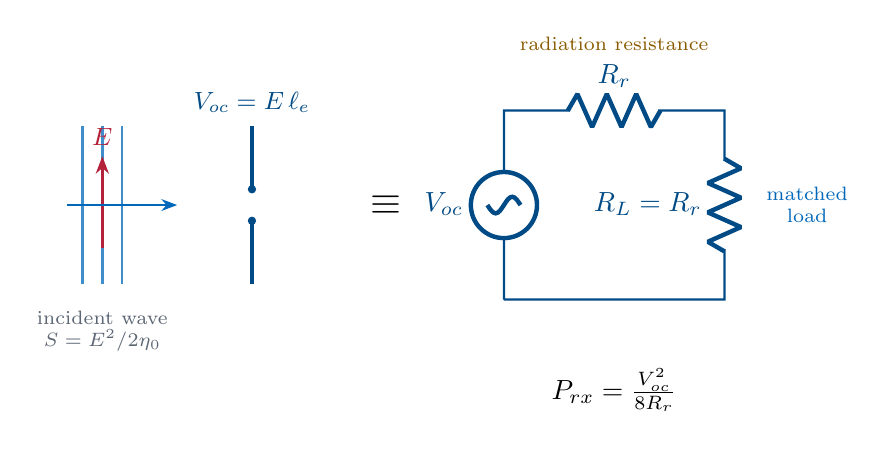
\begin{tikzpicture}[font=\sffamily, line width=0.8pt]
  % incident wave
  \foreach \x in {-0.25,0,0.25}{\draw[cblue!75,line width=1pt] (\x,-1)--(\x,1);}
  \draw[cred,-{Stealth[length=2.2mm]},line width=1.1pt] (0,-0.55)--(0,0.62)
        node[above,cred,font=\small\bfseries]{$E$};
  \draw[cblue,-{Stealth[length=2mm]}] (-0.45,0)--(0.95,0);
  \node[cink3,font=\scriptsize,align=center] at (0,-1.6){incident wave\\ $S=E^{2}/2\eta_{0}$};
  % receiving dipole, label lifted above
  \draw[navy,line width=1.5pt] (1.9,0.2)--(1.9,1.0);
  \draw[navy,line width=1.5pt] (1.9,-0.2)--(1.9,-1.0);
  \fill[navy] (1.9,0.2) circle(1.5pt) (1.9,-0.2) circle(1.5pt);
  \node[navy,font=\small,above] at (1.9,1.05){$V_{oc}=E\,\ell_{e}$};
  % equivalence
  \node[font=\Large\bfseries] at (3.6,0){$\equiv$};
  % Thevenin equivalent circuit
  \begin{scope}[xshift=5.1cm]
    \draw[navy]
      (0,-1.2) to[sV, l={$V_{oc}$}, invert] (0,1.2)
      to[R, l={$R_{r}$}] (2.8,1.2)
      to[R, l_={$R_{L}=R_{r}$}] (2.8,-1.2)
      -- (0,-1.2);
    \node[camber,font=\scriptsize] at (1.4,2.05){radiation resistance};
    \node[cblue,font=\scriptsize,align=center] at (3.85,0){matched\\ load};
  \end{scope}
  \node[font=\bfseries] at (6.5,-2.35){$P_{rx}=\frac{V_{oc}^{2}}{8R_{r}}$};
\end{tikzpicture}
\end{document}
